\documentclass[10pt,a4paper]{article}
\usepackage[utf8]{inputenc}
\usepackage[russian]{babel}
\usepackage[OT1]{fontenc}
\usepackage{amsmath}
\usepackage{amsfonts}
\usepackage{amssymb}
\usepackage{graphicx}
\graphicspath{{Images/}}
\usepackage[left=2cm,right=2cm,top=2cm,bottom=2cm]{geometry}
\usepackage{calc}
\usepackage{wrapfig}
\usepackage{setspace}
\usepackage{indentfirst}
\usepackage{subfigure}
\usepackage{multirow}
\usepackage{longtable}


\title{
Отчет о выполнении лабораторной работы 3.4.2

Закон Кюри-Вейсса
}

\author{Варламов Антоний, группа Б02-928}

\begin{document}

\maketitle

\newpage

	\section{Введение}
	
	\textit{Цель работы:} Изучение температурной зависимости магнитной восприимчивости ферромагнетика выше точки Кюри\\
	
	\textit{Оборудование и материалы:} катушка с образцом из гадолиния, термостат, частотомер, цифровой вольтметр, LC-автогенератор, термопара медь-константан. \\
	
	Для ферромагнетиков справедлив закон \textit{Кюри-Вейсса}:
	
	\begin{equation}
		\chi \sim \frac{1}{T - \Theta_{p}}
	\end{equation}
	
	где $\Theta_{p}$ -- температура, близкая к температуре Кюри.\\
	
	\begin{wrapfigure}[10]{r}{0.23\textwidth}
		\vspace{-1.5cm}
		\centering
		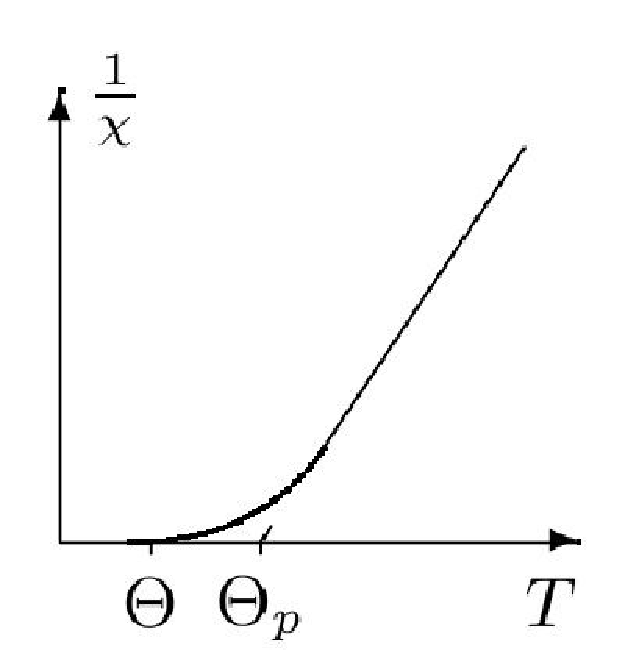
\includegraphics[width = 0.2\textwidth]{graph_return_chi_for_temp}
		\caption{График зависимости $\frac{1}{\chi}\left(T\right)$}
		\label{fig:graph_return_chi_for_temp}
	\end{wrapfigure}
	
	Данный закон хорошо работает в диапазоне температур:\\ $T \gg \Theta_{p}$. Для температур, близких к температуре Кюри вводят две величины:
	
	Собственно саму температуру Кюри (ферромагнитную) -- $\Theta$, и 
	
	Парамагнитную температуру Кюри -- $\Theta_{p}$.\\ В таком случае график зависимости величины, обратной магнитной восприимчивости образца изображен на рисунке (\ref{fig:graph_return_chi_for_temp}).
	
	Закон Кюри-Вейсса можно считать справедливым, если выполняется соотношение: 
	
	\begin{equation}
		\frac{1}{\chi} \sim \frac{1}{\tau^{2} - \tau^{2}_{0}} \sim \left(T - \Theta_{p}\right)
	\end{equation}
	
	\section{Параметры установки}
	
	\begin{figure}[h!]
		\begin{center}
			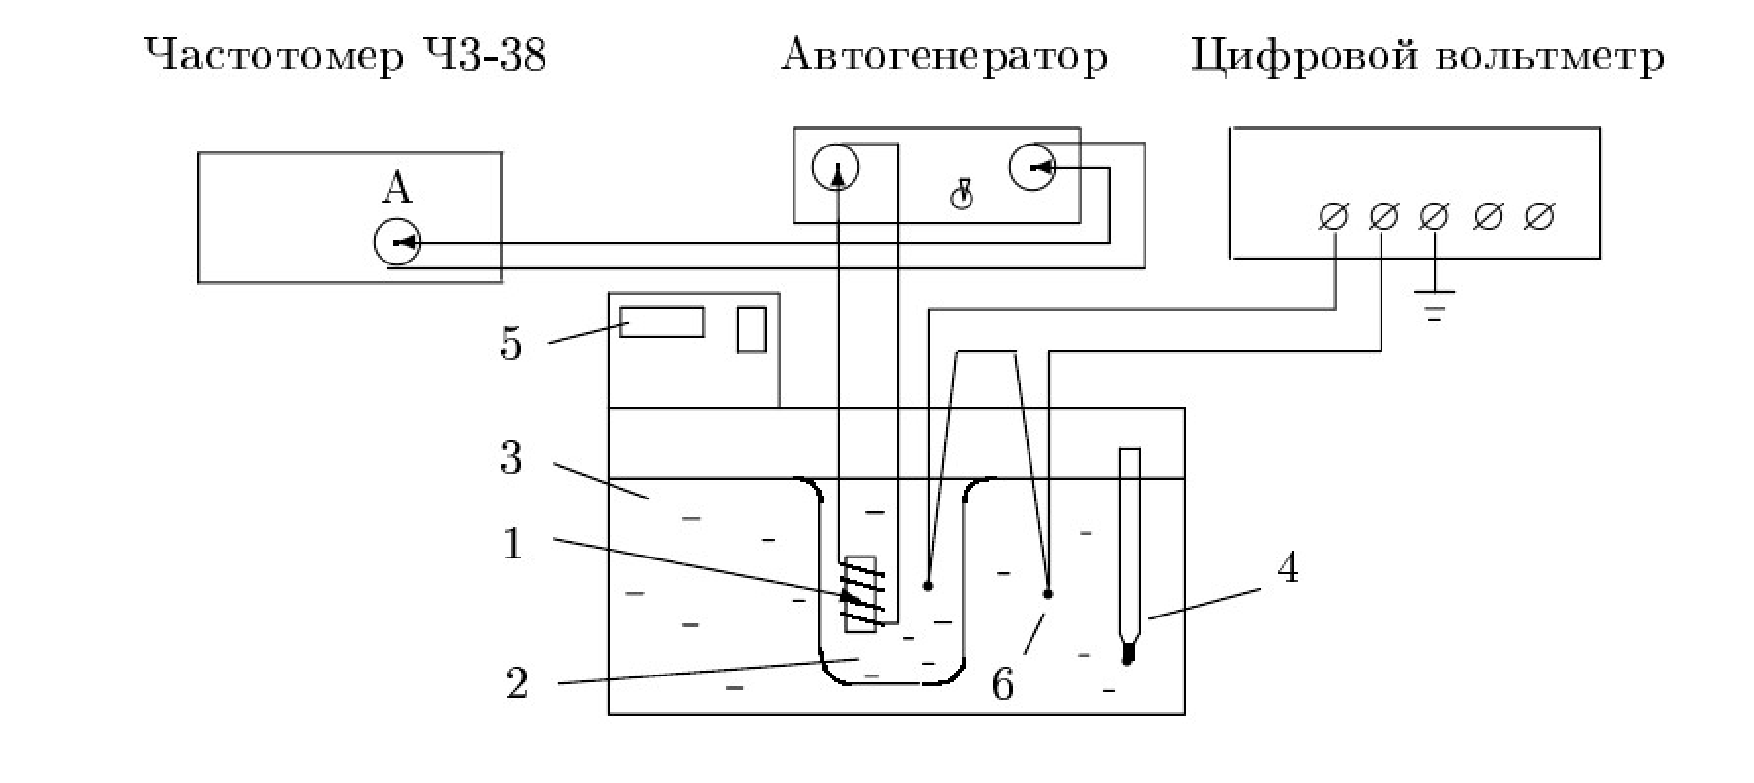
\includegraphics[width = 0.8\textwidth]{schem_of_facility}
			\label{fig:schem_of_facility}
			\caption{Схема установки. 1 - Катушка индуктивности с образцом из гадолиния, 2 - сосуд с трансформаторным маслом, 3 - вода, нагреваемая термостатом, 4 - ртутный термометр, 5 - блок термостата, 6 - термопара}
		\end{center}
	\end{figure}
	\newpage
	
	\section{Ход выполнения работы}
	
	\begin{longtable}[h!]{|l|l|l|l|l|l|l|}
\hline
№ измерения &
  $\tau,\, \text{мкс}$ &
  $\sigma_{\tau}^{\text{инстр}},\, \text{мкс}$ &
  $\Delta U, \, \text{мкВ}$ &
  $\sigma_{\Delta U}^{\text{случ}}, \,   \text{мкВ}$ &
  $T_{\text{воды}},\, ^{\circ}C$ &
  $\sigma_{T_{\text{воды}}}^{\text{случ}},\,   ^{\circ}C$ \\ \hline
\multicolumn{7}{|c|}{$T = 14^{\circ}\,C$}                                            \\ \hline
1 & 10,768 & 0,001 & 18 & 2                      & 14,01 & 0,01                      \\ \hline
\multicolumn{7}{|c|}{$T = 16^{\circ}\,C$}                                            \\ \hline
1 & 10,737 & 0,001 & 17 & 2                      & 16,02 & 0,01                      \\ \hline
\multicolumn{7}{|c|}{$T = 18^{\circ}\,C$}                                            \\ \hline
1 & 10,704 & 0,001 & 18 & 2                      & 18,00 & 0,01                      \\ \hline
\multicolumn{7}{|c|}{$T = 20^{\circ}\,C$}                                            \\ \hline
1 & 10,326 & 0,001 & 16 & 2                      & 20,00 & 0,01                      \\ \hline
2 & 10,317 & 0,001 & 15 & 2                      & 20,01 & 0,01                      \\ \hline
3 & 10,307 & 0,001 & 14 & 2                      & 20,01 & 0,01                      \\ \hline
4 & 10,302 & 0,001 & 13 & 2                      & 20,02 & 0,01                      \\ \hline
5 & 10,291 & 0,001 & 12 & 2                      & 20,02 & 0,01                      \\ \hline
6 & 10,284 & 0,001 & 11 & 2                      & 20,02 & 0,01                      \\ \hline
7 & 10,276 & 0,001 & 10 & 2                      & 20,02 & 0,01                      \\ \hline
8 & 10,270 & 0,001 & 9  & 2                      & 20,02 & 0,01                      \\ \hline
\multicolumn{7}{|c|}{$T = 22^{\circ}\,C$}                                            \\ \hline
1 & 9,985  & 0,001 & 15 & 2                      & 22,01 & 0,01                      \\ \hline
2 & 9,974  & 0,001 & 14 & 2                      & 22,02 & 0,01                      \\ \hline
3 & 9,962  & 0,001 & 14 & 2                      & 22,02 & 0,01                      \\ \hline
4 & 9,953  & 0,001 & 13 & 2                      & 22,02 & 0,01                      \\ \hline
5 & 9,544  & 0,001 & 12 & 2                      & 22,03 & 0,01                      \\ \hline
6 & 9,935  & 0,001 & 12 & 2                      & 22,04 & 0,01                      \\ \hline
7 & 9,928  & 0,001 & 11 & 2                      & 22,03 & 0,01                      \\ \hline
8 & 9,917  & 0,001 & 10 & 2                      & 22,04 & 0,01                      \\ \hline
\multicolumn{7}{|c|}{$T = 24^{\circ}\,C$}                                            \\ \hline
1 & 9,962  & 0,001 & 14 & 2 & 24,03 & 0,01 \\ \hline
2 & 9,606  & 0,001 & 14 & 2 & 24,03 & 0,01 \\ \hline
3 & 9,601  & 0,001 & 14 & 2 & 24,03 & 0,01 \\ \hline
4 & 9,597  & 0,001 & 13 & 2 & 24,04 & 0,01 \\ \hline
5 & 9,592  & 0,001 & 12 & 2 & 24,04 & 0,01 \\ \hline
6 & 9,581  & 0,001 & 11 & 2 & 24,05 & 0,01 \\ \hline
7 & 9,524  & 0,001 & 11 & 2 & 24,06 & 0,01 \\ \hline
8 & 9,480  & 0,001 & 11 & 2 & 24,06 & 0,01 \\ \hline
\multicolumn{7}{|c|}{$T = 26^{\circ}\,C$}                                            \\ \hline
1 & 9,440  & 0,001 & 17 & 2                      & 26,01 & 0,01                      \\ \hline
2 & 9,438  & 0,001 & 15 & 2                      & 26,01 & 0,01                      \\ \hline
3 & 9,435  & 0,001 & 16 & 2                      & 26,02 & 0,01                      \\ \hline
4 & 9,433  & 0,001 & 13 & 2                      & 26,03 & 0,01                      \\ \hline
5 & 9,430  & 0,001 & 13 & 2                      & 26,04 & 0,01                      \\ \hline
6 & 9,489  & 0,001 & 13 & 2                      & 26,04 & 0,01                      \\ \hline
7 & 9,427  & 0,001 & 12 & 2                      & 26,05 & 0,01                      \\ \hline
8 & 9,425  & 0,001 & 11 & 2                      & 26,05 & 0,01                      \\ \hline
\multicolumn{7}{|c|}{$T = 28^{\circ}\,C$}                                            \\ \hline
1 & 9,349  & 0,001 & 16 & 2                      & 28,01 & 0,01                      \\ \hline
2 & 9,347  & 0,001 & 16 & 2                      & 28,02 & 0,01                      \\ \hline
3 & 9,346  & 0,001 & 14 & 2                      & 28,02 & 0,01                      \\ \hline
4 & 9,345  & 0,001 & 13 & 2                      & 28,02 & 0,01                      \\ \hline
5 & 9,344  & 0,001 & 13 & 2                      & 28,03 & 0,01                      \\ \hline
6 & 9,343  & 0,001 & 13 & 2                      & 28,04 & 0,01                      \\ \hline
7 & 9,342  & 0,001 & 12 & 2                      & 28,04 & 0,01                      \\ \hline
8 & 9,341  & 0,001 & 11 & 2                      & 28,05 & 0,01                      \\ \hline
\multicolumn{7}{|c|}{$T = 30^{\circ}\,C$}                                            \\ \hline
1 & 9,295  & 0,001 & 15 & 2                      & 30,00 & 0,01                      \\ \hline
2 & 9,295  & 0,001 & 14 & 2                      & 30,01 & 0,01                      \\ \hline
3 & 9,294  & 0,001 & 11 & 2                      & 30,01 & 0,01                      \\ \hline
4 & 9,293  & 0,001 & 13 & 2                      & 30,02 & 0,01                      \\ \hline
5 & 9,292  & 0,001 & 13 & 2                      & 30,02 & 0,01                      \\ \hline
6 & 9,292  & 0,001 & 13 & 2                      & 30,03 & 0,01                      \\ \hline
7 & 9,291  & 0,001 & 12 & 2                      & 30,03 & 0,01                      \\ \hline
8 & 9,290  & 0,001 & 12 & 2                      & 30,04 & 0,01                      \\ \hline
\multicolumn{7}{|c|}{$T = 32^{\circ}\,C$}                                            \\ \hline
1 & 9,258  & 0,001 & 14 & 2                      & 32,01 & 0,01                      \\ \hline
2 & 9,257  & 0,001 & 14 & 2                      & 32,02 & 0,01                      \\ \hline
3 & 9,257  & 0,001 & 13 & 2                      & 32,03 & 0,01                      \\ \hline
4 & 9,256  & 0,001 & 14 & 2                      & 32,04 & 0,01                      \\ \hline
5 & 9,256  & 0,001 & 13 & 2                      & 32,04 & 0,01                      \\ \hline
6 & 9,255  & 0,001 & 12 & 2                      & 32,04 & 0,01                      \\ \hline
7 & 9,255  & 0,001 & 12 & 2                      & 32,05 & 0,01                      \\ \hline
8 & 9,254  & 0,001 & 12 & 2                      & 32,05 & 0,01                      \\ \hline
\multicolumn{7}{|c|}{$T = 34^{\circ}\,C$}                                            \\ \hline
1 & 9,231  & 0,001 & 16 & 2                      & 34,00 & 0,01                      \\ \hline
2 & 9,230  & 0,001 & 15 & 2                      & 34,00 & 0,01                      \\ \hline
3 & 9,230  & 0,001 & 14 & 2                      & 34,01 & 0,01                      \\ \hline
4 & 9,229  & 0,001 & 15 & 2                      & 34,01 & 0,01                      \\ \hline
5 & 9,229  & 0,001 & 13 & 2                      & 34,02 & 0,01                      \\ \hline
6 & 9,229  & 0,001 & 14 & 2                      & 34,02 & 0,01                      \\ \hline
7 & 9,228  & 0,001 & 13 & 2                      & 34,03 & 0,01                      \\ \hline
8 & 9,228  & 0,001 & 12 & 2                      & 34,03 & 0,01                      \\ \hline
\multicolumn{7}{|c|}{$T = 36^{\circ}\,C$}                                            \\ \hline
1 & 9,210  & 0,001 & 15 & 2                      & 36,00 & 0,01                      \\ \hline
2 & 9,209  & 0,001 & 15 & 2                      & 36,00 & 0,01                      \\ \hline
3 & 9,209  & 0,001 & 14 & 2                      & 36,01 & 0,01                      \\ \hline
4 & 9,209  & 0,001 & 14 & 2                      & 36,02 & 0,01                      \\ \hline
5 & 9,209  & 0,001 & 14 & 2                      & 36,02 & 0,01                      \\ \hline
6 & 9,208  & 0,001 & 12 & 2                      & 36,02 & 0,01                      \\ \hline
7 & 9,208  & 0,001 & 11 & 2                      & 36,03 & 0,01                      \\ \hline
8 & 9,208  & 0,001 & 11 & 2                      & 36,03 & 0,01                      \\ \hline
\multicolumn{7}{|c|}{$T = 38^{\circ}\,C$}                                            \\ \hline
1 & 9,194  & 0,001 & 16 & 2                      & 38,00 & 0,01                      \\ \hline
2 & 9,194  & 0,001 & 16 & 2                      & 38,00 & 0,01                      \\ \hline
3 & 9,194  & 0,001 & 15 & 2                      & 38,01 & 0,01                      \\ \hline
4 & 9,193  & 0,001 & 15 & 2                      & 38,01 & 0,01                      \\ \hline
5 & 9,194  & 0,001 & 14 & 2                      & 38,01 & 0,01                      \\ \hline
6 & 9,194  & 0,001 & 13 & 2                      & 38,02 & 0,01                      \\ \hline
7 & 9,193  & 0,001 & 13 & 2                      & 38,02 & 0,01                      \\ \hline
8 & 9,193  & 0,001 & 12 & 2                      & 38,03 & 0,01                      \\ \hline
\multicolumn{7}{|c|}{$T = 40^{\circ}\,C$}                                            \\ \hline
1 & 9,182  & 0,001 & 15 & 2                      & 40,00 & 0,01                      \\ \hline
2 & 9,181  & 0,001 & 15 & 2                      & 40,00 & 0,01                      \\ \hline
3 & 9,181  & 0,001 & 14 & 2                      & 40,01 & 0,01                      \\ \hline
4 & 9,181  & 0,001 & 13 & 2                      & 40,02 & 0,01                      \\ \hline
5 & 9,181  & 0,001 & 12 & 2                      & 40,01 & 0,01                      \\ \hline
6 & 9,181  & 0,001 & 12 & 2                      & 40,02 & 0,01                      \\ \hline
7 & 9,180  & 0,001 & 12 & 2                      & 40,03 & 0,01                      \\ \hline
8 & 9,180  & 0,001 & 11 & 2                      & 40,03 & 0,01                      \\ \hline 

\caption{Результаты измерения зависимости периода колебаний в LC-контуре от температуры}
\end{longtable}

\newpage
	
	\section{Обработка полученных данных}
	
	Для подтверждения закона Кюри-Вейсса необходимо построить график зависимости $\frac{1}{\tau^{2} - \tau^{2}_{0}} = f\left(T\right);$.
	
	Для этого оценим погрешности измеряемых величин.
	
	\subsection{Определение погрешности измерения периода колебаний}
	
		Для определения величины погрешности измерения периода определим природу данной погрешности. Так как период измеряется непосредственно с помощью частотомера, то погрешность измерения периода -- погрешность измерительного инструмента и случайная погрешность. определим случайную погрешность измерения периода -- $\sigma_{\tau}^{\text{случ}}$:
		
		\begin{table}[h!]
\centering
\begin{tabular}{|l|l|l|l|l|}
\hline
$T, ^{\circ} C$ & $\overline{\tau}, \text{мкс}$ & $\sigma_{\tau}^{\text{случ}}, \text{мкс}$ & $\sigma_{\tau}^{\text{приб}}, \text{мкс}$ & $\sigma_{\tau}, \text{мкс}$ \\ \hline
14 & 10,768 & 0,020 & 0,001 & 0,020 \\ \hline
16 & 10,737 & 0,020 & 0,001 & 0,020 \\ \hline
18 & 10,704 & 0,020 & 0,001 & 0,020 \\ \hline
20 & 10,296 & 0,019 & 0,001 & 0,019 \\ \hline
22 & 9,900  & 0,136 & 0,001 & 0,136 \\ \hline
24 & 9,618  & 0,136 & 0,001 & 0,136 \\ \hline
26 & 9,439  & 0,019 & 0,001 & 0,019 \\ \hline
28 & 9,345  & 0,002 & 0,001 & 0,003 \\ \hline
30 & 9,293  & 0,002 & 0,001 & 0,002 \\ \hline
32 & 9,256  & 0,001 & 0,001 & 0,002 \\ \hline
34 & 9,229  & 0,001 & 0,001 & 0,001 \\ \hline
36 & 9,209  & 0,001 & 0,001 & 0,001 \\ \hline
38 & 9,194  & 0,000 & 0,001 & 0,001 \\ \hline
40 & 9,181  & 0,000 & 0,001 & 0,001 \\ \hline
\end{tabular}
\caption{Значение погрешностей для величины периода}
\label{tab:errors_period}
\end{table}

		Как видно из таблицы (\ref{tab:errors_period}) наибольшее отклонение от среднего значения было зафиксировано в диапазоне $22-24 ^{\circ}\, C$. Значение относительной погрешности при этом достигает $\varepsilon_{\tau, \text{макс}} = \frac{\sigma_{\tau}}{\tau} \approx 10^{-2}$, что является приемлемым результатом.
		
		Получив значение погрешности прямого измерения периода, можно оценить погрешность косвенного измерения величины $\frac{1}{\tau^{2} - \tau^{2}_{0}}$. Для этого рассмотрим функцию:
		
		\begin{equation}
			f\left(\tau\right) = \frac{1}{\tau^{2} - \tau^{2}_{0}}
		\end{equation}	
		
		Для погрешности косвенного измерения воспользуемся формулой:
		
		\begin{equation}
			\sigma_{f}  = \sqrt{\left(\frac{\partial f}{\partial \tau}\left(\tau\right)\right)^{2} \cdot \sigma^{2}_{\tau}}
		\end{equation}
		
		\begin{equation}
			\sigma_{f}  = \sqrt{\frac{4\tau^{2}}{\left(\tau^{2} - \tau^{2}_{0}\right)^{4}}\sigma_{\tau}}
		\end{equation}
		
		\begin{equation}
			\sigma_{f}  = \frac{2\tau \sigma_{\tau}}{\left(\tau^{2} - \tau^{2}_{0}\right)^{2}}
		\end{equation}
		

		\begin{table}[h!]
\hspace{-1cm}
\begin{tabular}{|l|l|l|l|l|l|l|l|l|l|l|l|l|l|l|}
\hline
$\tau, \text{мкс}$               & 10,768 & 10,737 & 10,704 & 10,296 & 9,900 & 9,618 & 9,439 & 9,345 & 9,293 & 9,256 & 9,229 & 9,209 & 9,194 & 9,181 \\ \hline
$\sigma_{f}$          & 0,001  & 0,001  & 0,001  & 0,001  & 0,010 & 0,023 & 0,007 & 0,002 & 0,002 & 0,002 & 0,002 & 0,002 & 0,003 & 0,003 \\ \hline
$f\left(\tau\right)$ & 0,029  & 0,030  & 0,031  & 0,041  & 0,062 & 0,094 & 0,137 & 0,181 & 0,220 & 0,259 & 0,297 & 0,335 & 0,369 & 0,404 \\ \hline
\end{tabular}
\caption{Погрешность косвенных измерений}
\label{tab:error_of_f}
\end{table}

	Как видно из таблицы (\ref{tab:error_of_f}), относительная погрешность косвенных измерений не превосходит $0,25$, что говорит о приемлемой точности измерений.
	
	\subsection{Определение погрешности измерения температуры.}
	
	Для определения погрешности измерения температуры необходимо указать, каким образом происходит измерение температуры образца, так как это косвенное измерение.
	
	Для температуры образца справедлива формула:
	
	\begin{equation}
		T_{Gd} = T_{\text{термостата}} + kU_{\text{термопары}}
	\end{equation}
	
	В соответствии с данной формулой можем записать формулу для определения величины погрешности косвенного измерения:
	
	\begin{equation}
		\sigma_{T_{Gd}} = \sqrt{\left(\left(\frac{\partial f}{\partial T_{\text{термостата}}}\right)\cdot \sigma_{T_{\text{термостата}}}\right)^{2} + \left(\left(\frac{\partial f}{\partial U}\right)\cdot \sigma_{U}\right)^{2}}
	\end{equation}
	
	\begin{equation}
		\sigma_{T_{Gd}} = \sqrt{\sigma_{T}^{2} + k^{2}\sigma_{U}^{2}}
	\end{equation}	
	
	\begin{table}[h!]
\hspace{-1cm}
\begin{tabular}{|l|l|l|l|l|l|l|l|l|l|l|l|l|l|l|}
\hline
$\tau, \text{мкс}$               & 10,768 & 10,737 & 10,704 & 10,296 & 9,900 & 9,618 & 9,439 & 9,345 & 9,293 & 9,256 & 9,229 & 9,209 & 9,194 & 9,181 \\ \hline
$\sigma_{f}$          & 0,001  & 0,001  & 0,001  & 0,001  & 0,010 & 0,023 & 0,007 & 0,002 & 0,002 & 0,002 & 0,002 & 0,002 & 0,003 & 0,003 \\ \hline
$f\left(\tau\right)$ & 0,029 & 0,030 & 0,031 & 0,041 & 0,062 & 0,094 & 0,137 & 0,181 & 0,220 & 0,259 & 0,297 & 0,335 & 0,369 & 0,404 \\ \hline
$T_{Gd}\,  ^{\circ}\, C$ & 14,4   & 16,4   & 18,4   & 20,3   & 22,3  & 24,3  & 26,3  & 28,3  & 30,3  & 32,3  & 34,3  & 36,3  & 38,3  & 40,3  \\ \hline
$\sigma_{T_{Gd}}\,  ^{\circ}\, C$    & 0,5    & 0,5    & 0,5    & 0,7    & 0,6   & 0,6   & 0,7   & 0,6   & 0,6   & 0,5   & 0,6   & 0,6   & 0,6   & 0,6	   \\ \hline
\end{tabular}
\caption{Результаты определения погрешности косвенных вычислений температуры и периода колебаний образца}
\label{tab:final_data}
\end{table}			

	\begin{figure}[h!]
		\begin{center}
			\begin{minipage}[h]{0.49\linewidth}
				\hspace{-2,5cm}
				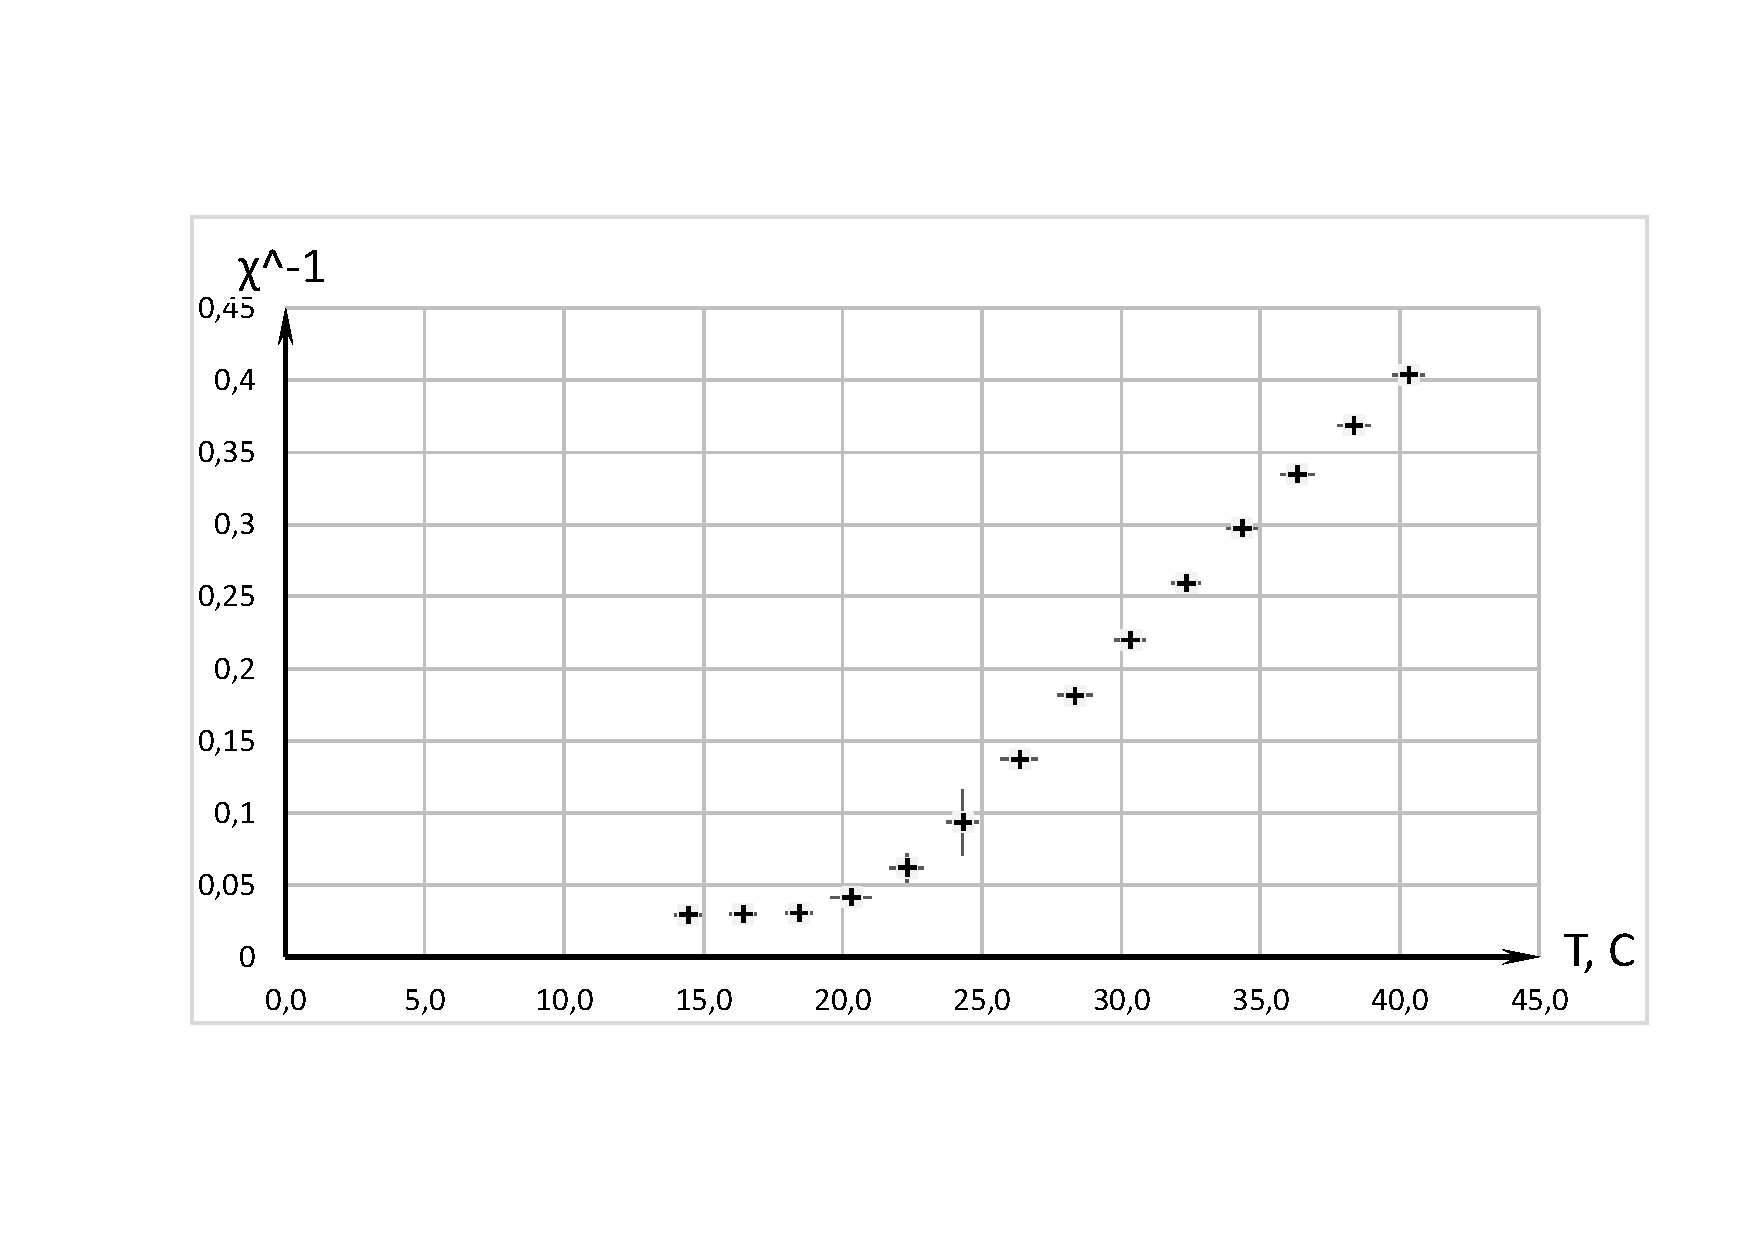
\includegraphics[width=1.4\linewidth]{Graph_final_1}
				\caption{График зависимости $\frac{1}{\tau^{2} - \tau^{2}_{0}} = f\left(T\right)$} %% подпись к рисунку
				\label{ris:Graph_final_1} %% метка рисунка для ссылки на него
			\end{minipage}
		\hfill
			\begin{minipage}[h]{0.49\linewidth}
				\hspace{-1,5cm}
				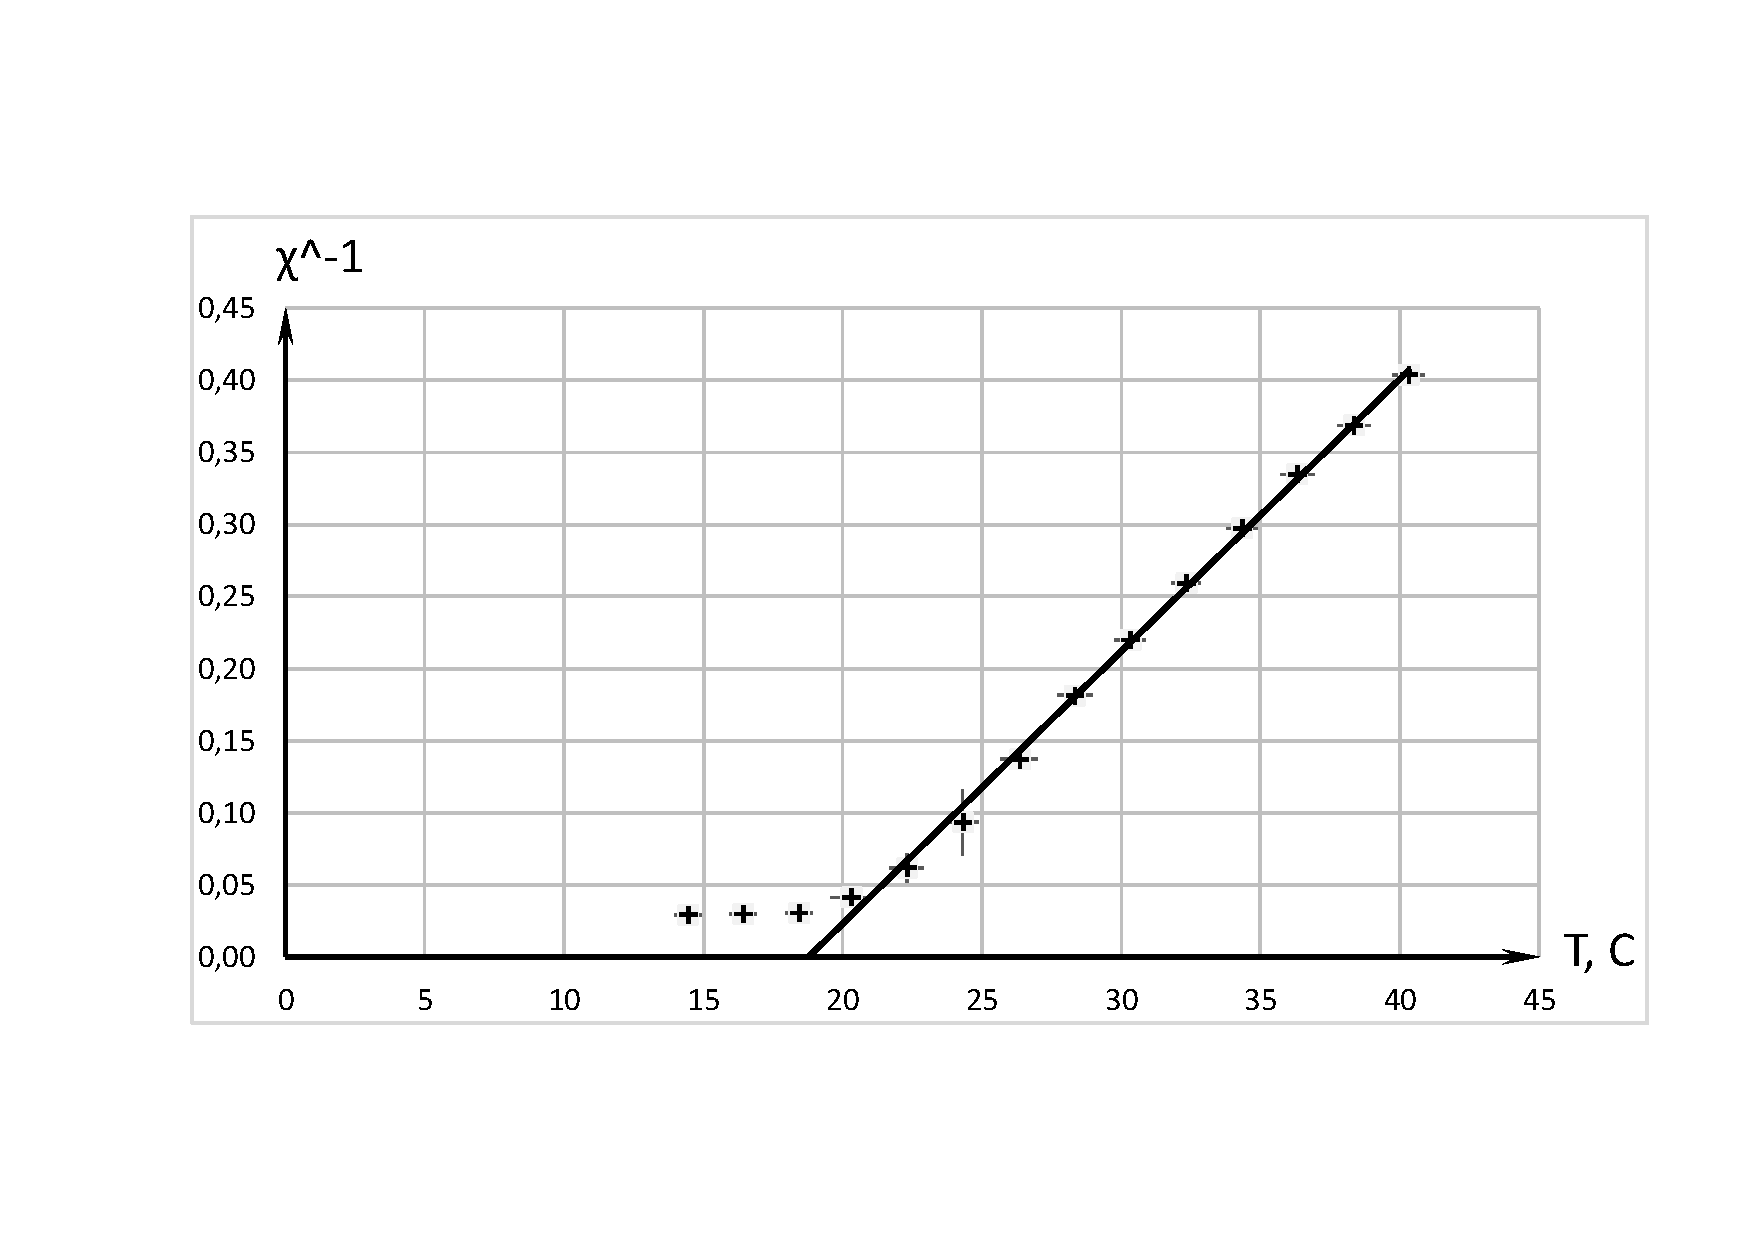
\includegraphics[width=1.4\linewidth]{Graph_final_2}
				\caption{Экстраполяция графика линейной функцией}
				\label{ris:Graph_final_2}
			\end{minipage}
		\end{center}
	\end{figure}
	
	С помощью МНК по данным таблиц (\ref{tab:errors_period}, \ref{tab:error_of_f}, \ref{tab:final_data}) получаем итоговые параметры температуры Кюри для Гадолиния:
	
	\begin{equation}
		\Theta_{Gd, p} = 18,0 \pm 1,0\, ^{\circ}\,C
	\end{equation}	
	
	\newpage
	 
					 
	\section{Итоги}
	
	\begin{enumerate}
		\item В ходе работы был экспериментально подтвержден закон Кюри-Вейсса для металла гадолиния. Была найдена температура Кюри (парамагнитная температура Кюри):
		
			$$\Theta_{Gd, p} = 18,0 \pm 1,0 \, ^{\circ}\,C$$
			
			Полученное значение согласуется с известными экспериментальными данными $\Theta_{Gd, p} \approx 290 K$.
		\item Определена погрешность полученного результата. Погрешность составила $\varepsilon \approx 7 \%$. Основной вклад в погрешность внесла неточность данных, полученных при температурах, близких к температуре Кюри. Неточность связана с проблемами, возникшими при использовании оборудования для проведения эксперимента.
		
		\item Анализ погрешностей показал, что достаточно проводить измерения температуры с точностью до 0,1, ЭДС в термопаре с точностью $\sim 5 \cdot 10^{-6}$ В. Наибольший вклад в погрешность конечного результата вносит погрешность косвенных измерений промежуточных величин.
	\end{enumerate}

\end{document}